\usecasegenerico{Effettua accesso}
\label{usecase:Effettua accesso}

\begin{figure}[h]
	\centering
	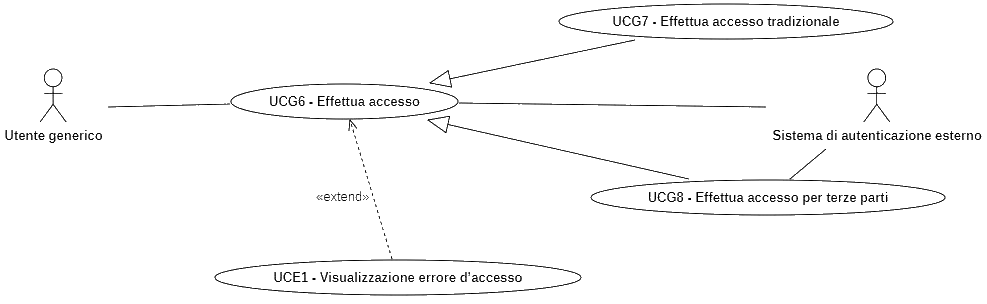
\includegraphics[width=0.9\textwidth]{./uml/UCG6-7-8.png} 
	\caption{Effettua accesso}
	\label{fig:UCG6-7-8}
  \end{figure}

\begin{itemize}
	\item \textbf{Descrizione:} Un Utente generico decide di accedere alla \textit{web app$^G$}, scegliendo tra due opzioni:
	\begin{itemize}
		\item Accesso tramite inserimento di \textit{email} e \textit{password}.
		\item Accesso tramite un sistema di terze parti.
	\end{itemize}
	In caso di fallimento dell'autenticazione, l'Utente generico deve reinserire le credenziali.

	\item \textbf{Attore principale:} Utente generico.
	\item \textbf{Attore secondario:} Sistema di autenticazione esterno$^G$.
	\item \textbf{Precondizione:}
	      Un Utente generico è connesso al Sistema ed è in possesso di un \textit{account}.

	\item \textbf{Postcondizioni:}
		\begin{itemize}      
			\item L'Utente generico è stato identificato dal Sistema come uno solo dei seguenti utenti:
	      		\begin{itemize}
		      		\item Utente ristoratore.
		      		\item Utente base.
	      		\end{itemize}
		  	\item L'Utente autenticato viene reindirizzato alla pagina \textit{Home} di pertinenza.
		\end{itemize}

	\item \textbf{Scenario principale:}
	      \begin{enumerate}
		      \item L'Utente generico seleziona la modalità di accesso: 

			  \begin{itemize}
				\item Accesso per terze parti (vedi \autoref{usecase:Effettua accesso per terze parti}).
				\item Accesso tradizionale (vedi \autoref{usecase:Effettua accesso tradizionale}).
			  \end{itemize}

		      \item Il Sistema verifica se l'Utente generico è un Utente ristoratore oppure Utente base;
		      \item L'Utente autenticato viene reindirizzato alla \textit{Home} corrispondente al tipo di \textit{account}.
	      \end{enumerate}
		
	\item \textbf{Scenario secondario:}
		\begin{enumerate}
			\item L'accesso fallisce (vedi \autoref{usecase:Visualizzazione errore d'accesso});
			\item L'Utente generico viene nuovamente indirizzato alla pagina di accesso.
		\end{enumerate}	
	\end{itemize}
